\chapter{Enumeration of \glsfmtlongpl{dof}: Demonstration}
\label{app::enumeration}
\glsresetall

This section delivers a visual demonstration of the enumeration algorithm for \glspl{dof} on the corresponding benchmark from Sec.~\ref{sec:enumeration}.

The test case is composed out of four adjacent cells, from which two catty-cornered ones are assigned to the same Lagrangian finite element of either order two or four. The mesh is divided into two subdomains, each containing two neighboring cells of different finite elements. In this configuration, cells are either locally owned or ghost cells. The setup of the benchmark is shown in Fig.~\ref{fig:enumbenchmark}. %Fig.~\ref{fig:enumdemosetup}.

This scenario covers all combinations of adjacent finite elements in the parallel \hp-adaptive context, which makes it a perfect minimal example. Here, we encounter neighboring cells with similar and different finite elements on the same and another subdomain, with dominating finite elements on either a locally owned or a ghost cell.

For the bulk enumeration of locally owned \glspl{dof}, we comply to the scheme that is used in the \dealii{} library. We summarize how \glspl{dof} on Lagrange elements are enumerated in two dimensions: We iterate over all cells following a Z-order or Morton space filling curve, starting from the bottom left corner. On each cell, we first enumerate all \glspl{dof} on vertices in the same Z-order. Next, all interfaces in the order left, right, bottom, top are enumerated, each starting from the bottom left corner. Finally, all \glspl{dof} inside the quadrilateral are enumerated row-wise starting from the bottom left, i.e., lexicographically. \textcite{dealiifeq}

We apply the algorithm step-by-step on this particular example and present its intermediate states in Fig.~\ref{fig:enumdemosteps}.

{% scope of variables
\let\oldthesubfigure\thesubfigure
\renewcommand{\thesubfigure}{Phase \arabic{subfigure}}

\def\Length{1}
\def\Radius{0.03}

\begin{figure}
\centering
\begin{subfigure}{\textwidth}
  \resizebox{\textwidth}{!}{
    
\begin{tikzpicture}[scale=3.3]
  \fill[color=green] (0, 0) rectangle (2*\Length, \Length);

  \LagrangeCell{0}{0}{\Length}{\Radius}{2}
    {{0,1,2,3,4,5,6,7,8}};
  \LagrangeCell{\Length}{0}{\Length}{\Radius}{4}
    {{9,10,11,12,13,14,15,16,17,18,19,20,21,22,23,24,25,26,27,28,29,30,31,32,33}};
  \LagrangeCell{0}{\Length}{\Length}{\Radius}{4}
    {{"i","i","i","i","i","i","i","i","i","i","i","i","i","i","i","i","i","i","i","i","i","i","i","i","i"}};
  \LagrangeCell{\Length}{\Length}{\Length}{\Radius}{3}
    {{"i","i","i","i","i","i","i","i","i","i","i","i","i","i","i","i"}};
\end{tikzpicture}

    \hfill{}
    
\begin{tikzpicture}[scale=3.3]
  \fill[color=green] (0, \Length) rectangle (2*\Length, 2*\Length);
  
  \LagrangeCell{0}{0}{\Length}{\Radius}{2}
    {{"i","i","i","i","i","i","i","i","i"}};
  \LagrangeCell{\Length}{0}{\Length}{\Radius}{4}
    {{"i","i","i","i","i","i","i","i","i","i","i","i","i","i","i","i","i","i","i","i","i","i","i","i","i"}};
  \LagrangeCell{0}{\Length}{\Length}{\Radius}{4}
    {{0,1,2,3,4,5,6,7,8,9,10,11,12,13,14,15,16,17,18,19,20,21,22,23,24}};
  \LagrangeCell{\Length}{\Length}{\Length}{\Radius}{2}
    {{25,26,27,28,29,30,31,32,33}};
\end{tikzpicture}

  }
  \caption{Local enumeration.}
\end{subfigure}
\begin{subfigure}{\textwidth}
  \resizebox{\textwidth}{!}{
    \begin{tikzpicture}[scale=3.3]
  \LagrangeCell{0}{0}{\Length}{\Radius}{2}
    {{0,1,2,3,4,5,6,7,8}};
  \LagrangeCell{\Length}{0}{\Length}{\Radius}{4}
    {{9,10,11,12,13,14,15,16,17,18,19,20,21,22,23,24,25,26,27,28,29,30,31,32,33}};
  \LagrangeCell{0}{\Length}{\Length}{\Radius}{4}
    {{"i","i","i","i","i","i","i","i","i","i","i","i","i","i","i","i","i","i","i","i","i","i","i","i","i"}};
  \LagrangeCell{\Length}{\Length}{\Length}{\Radius}{2}
    {{"i","i","i","i","i","i","i","i","i","i","i","i","i","i","i","i"}};
\end{tikzpicture}
    \hfill{}
    
\begin{tikzpicture}[scale=3.3]
  \fill[color=green] (\Length - 0.15, \Length) rectangle (\Length + 0.15, \Length + 0.15);
  
  \LagrangeCell{0}{0}{\Length}{\Radius}{2}
    {{"i","i","i","i","i","i","i","i","i"}};
  \LagrangeCell{\Length}{0}{\Length}{\Radius}{4}
    {{"i","i","i","i","i","i","i","i","i","i","i","i","i","i","i","i","i","i","i","i","i","i","i","i","i"}};
  \LagrangeCell{0}{\Length}{\Length}{\Radius}{4}
    {{0,"i",2,3,4,5,6,7,8,9,10,11,12,13,14,15,16,17,18,19,20,21,22,23,24}};
  \LagrangeCell{\Length}{\Length}{\Length}{\Radius}{2}
    {{"i",26,27,28,29,30,31,32,33}};
\end{tikzpicture}

  }
  \caption{Tie-break.}
\end{subfigure}
\begin{subfigure}{\textwidth}
  \resizebox{\textwidth}{!}{
    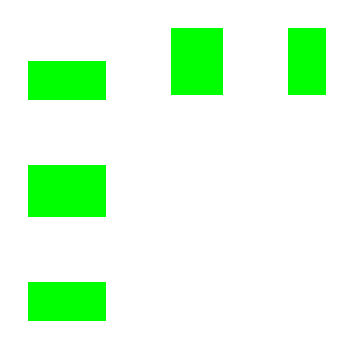
\begin{tikzpicture}[scale=3.3]
  \fill[color=green] (\Length - 0.15, 0) rectangle (\Length + 0.15, 0.15);
  \fill[color=green] (\Length - 0.15, 0.5*\Length - 0.1) rectangle (\Length + 0.15, 0.5*\Length + 0.1);
  \fill[color=green] (\Length - 0.15, \Length - 0.15) rectangle (\Length + 0.15, \Length);
  
  \fill[color=green] (1.5*\Length - 0.1, \Length - 0.13) rectangle (1.5*\Length + 0.1, \Length + 0.13);
  \fill[color=green] (2*\Length - 0.15, \Length - 0.13) rectangle (2*\Length, \Length + 0.13);
  
  \LagrangeCell{0}{0}{\Length}{\Radius}{2}
    {{0,1,2,3,4,5,6,7,8}};
  \LagrangeCell{\Length}{0}{\Length}{\Radius}{4}
    {{1,10,3,"i",13,5,15,16,17,18,19,20,21,22,"i",24,25,26,27,28,29,30,31,32,33}};
  \LagrangeCell{0}{\Length}{\Length}{\Radius}{4}
    {{"i","i","i","i","i","i","i","i","i","i","i","i","i","i","i","i","i","i","i","i","i","i","i","i","i"}};
  \LagrangeCell{\Length}{\Length}{\Length}{\Radius}{2}
    {{"i","i","i","i","i","i","i","i","i","i","i","i","i","i","i","i"}};
\end{tikzpicture}
    \hfill{}
    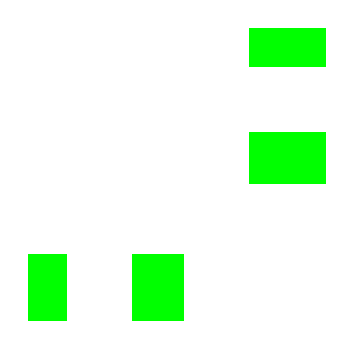
\begin{tikzpicture}[scale=3.3]
  \fill[color=green] (\Length - 0.15, 1.5*\Length - 0.1) rectangle (\Length + 0.15, 1.5*\Length + 0.1);
  \fill[color=green] (\Length - 0.15, 2*\Length - 0.15) rectangle (\Length + 0.15, 2*\Length);
  
  \fill[color=green] (0, \Length - 0.13) rectangle (0.15, \Length + 0.13);
  \fill[color=green] (0.5*\Length - 0.1, \Length - 0.13) rectangle (0.5*\Length + 0.1, \Length + 0.13);
  
  \LagrangeCell{0}{0}{\Length}{\Radius}{2}
    {{"i","i","i","i","i","i","i","i","i"}};
  \LagrangeCell{\Length}{0}{\Length}{\Radius}{4}
    {{"i","i","i","i","i","i","i","i","i","i","i","i","i","i","i","i","i","i","i","i","i","i","i","i","i"}};
  \LagrangeCell{0}{\Length}{\Length}{\Radius}{4}
    {{"i","i",2,27,4,5,6,7,29,9,10,"i",12,13,14,15,16,17,18,19,20,21,22,23,24}};
  \LagrangeCell{\Length}{\Length}{\Length}{\Radius}{2}
    {{"i",26,27,28,29,30,31,32,33}};
\end{tikzpicture}
  }
  \caption{Unification.}
\end{subfigure}
\caption[Step-by-step demonstration of the enumeration algorithm for \glsfmtlongpl{dof} on the benchmark.]{Step-by-step demonstration of the enumeration algorithm for \glspl{dof} on the benchmark. Changes made at each step are highlighted. The left domain corresponds to the full mesh of the \gls{mpi} process with rank 0, the right one belongs to the one with rank 1.}
\label{fig:enumdemosteps}
\end{figure}

\begin{figure}
\ContinuedFloat
\begin{subfigure}{\textwidth}
  \resizebox{\textwidth}{!}{
    
\begin{tikzpicture}[scale=3.3]
  \fill[color=green] (0, 0) rectangle (2*\Length, \Length);
  
  \fill[white] (1.5*\Length - 0.1, \Length - 0.13) rectangle (1.5*\Length + 0.1, \Length + 0.13);
  \fill[white] (2*\Length - 0.15, \Length - 0.13) rectangle (2*\Length, \Length + 0.13);
  
  \LagrangeCell{0}{0}{\Length}{\Radius}{2}
    {{0,1,2,3,4,5,6,7,8}};
  \LagrangeCell{\Length}{0}{\Length}{\Radius}{4}
    {{1,9,3,"i",10,5,11,12,13,14,15,16,17,18,"i",19,20,21,22,23,24,25,26,27,28}};
  \LagrangeCell{0}{\Length}{\Length}{\Radius}{4}
    {{"i","i","i","i","i","i","i","i","i","i","i","i","i","i","i","i","i","i","i","i","i","i","i","i","i"}};
  \LagrangeCell{\Length}{\Length}{\Length}{\Radius}{2}
    {{"i","i","i","i","i","i","i","i","i","i","i","i","i","i","i","i"}};
\end{tikzpicture}
    \hfill{}
    
\begin{tikzpicture}[scale=3.3]
  \fill[color=green] (0, \Length) rectangle (2*\Length, 2*\Length);
  
  \fill[white] (\Length - 0.15, \Length) rectangle (\Length + 0.15, \Length + 0.15);
  \fill[white] (0, \Length - 0.13) rectangle (0.15, \Length + 0.13);
  \fill[white] (0.5*\Length - 0.1, \Length - 0.13) rectangle (0.5*\Length + 0.1, \Length + 0.13);
  
  \LagrangeCell{0}{0}{\Length}{\Radius}{2}
    {{"i","i","i","i","i","i","i","i","i"}};
  \LagrangeCell{\Length}{0}{\Length}{\Radius}{4}
    {{"i","i","i","i","i","i","i","i","i","i","i","i","i","i","i","i","i","i","i","i","i","i","i","i","i"}};
  \LagrangeCell{0}{\Length}{\Length}{\Radius}{4}
    {{"i","i",29,50,30,31,32,33,52,34,35,"i",36,37,38,39,40,41,42,43,44,45,46,47,48}};
  \LagrangeCell{\Length}{\Length}{\Length}{\Radius}{2}
    {{"i",49,50,51,52,53,54,55,56}};
\end{tikzpicture}
  }
  \caption{Global re-enumeration.}
\end{subfigure}
\begin{subfigure}{\textwidth}
  \resizebox{\textwidth}{!}{
    
\begin{tikzpicture}[scale=3.3]
  \fill[color=green] (0,\Length) rectangle (2*\Length, 2*\Length);
  
  \fill[white] (\Length - 0.15, \Length) rectangle (\Length + 0.15, \Length + 0.15);
  \fill[white] (0, \Length - 0.13) rectangle (0.15, \Length + 0.13);
  \fill[white] (0.5*\Length - 0.1, \Length - 0.13) rectangle (0.5*\Length + 0.1, \Length + 0.13);
  
  \LagrangeCell{0}{0}{\Length}{\Radius}{2}
    {{0,1,2,3,4,5,6,7,8}};
  \LagrangeCell{\Length}{0}{\Length}{\Radius}{4}
    {{1,9,3,"i",10,5,11,12,13,14,15,16,17,18,"i",19,20,21,22,23,24,25,26,27,28}};
  \LagrangeCell{0}{\Length}{\Length}{\Radius}{4}
    {{"i","i",29,30,31,32,33,34,35,36,37,"i",38,39,40,41,42,43,44,45,46,47,48,49,50}};
  \LagrangeCell{\Length}{\Length}{\Length}{\Radius}{2}
    {{"i",51,30,52,35,53,54,55,56}};
\end{tikzpicture}
    \hfill{}
    
\begin{tikzpicture}[scale=3.3]
  \fill[color=green] (0,0) rectangle (2*\Length, \Length);
  
  \fill[white] (1.5*\Length - 0.1, \Length - 0.13) rectangle (1.5*\Length + 0.1, \Length + 0.13);
  \fill[white] (2*\Length - 0.15, \Length - 0.13) rectangle (2*\Length, \Length + 0.13);
  
  \LagrangeCell{0}{0}{\Length}{\Radius}{2}
    {{0,1,2,3,4,5,6,7,8}};
  \LagrangeCell{\Length}{0}{\Length}{\Radius}{4}
    {{1,9,3,"i",10,5,11,12,13,14,15,16,17,18,"i",19,20,21,22,23,24,25,26,27,28}};
  \LagrangeCell{0}{\Length}{\Length}{\Radius}{4}
    {{"i","i",29,50,30,31,32,33,52,34,35,"i",36,37,38,39,40,41,42,43,44,45,46,47,48}};
  \LagrangeCell{\Length}{\Length}{\Length}{\Radius}{2}
    {{"i",49,50,51,52,53,54,55,56}};
\end{tikzpicture}
  }
  \caption{Ghost exchange.}
\end{subfigure}
\begin{subfigure}{\textwidth}
  \resizebox{\textwidth}{!}{
    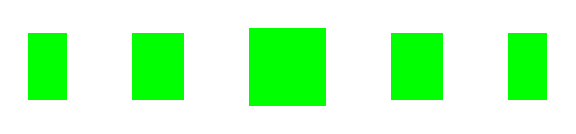
\begin{tikzpicture}[scale=3.3]
  \fill[color=green] (0, \Length - 0.13) rectangle (0.15, \Length + 0.13);
  \fill[color=green] (0.5*\Length - 0.1, \Length - 0.13) rectangle (0.5*\Length + 0.1, \Length + 0.13);
  \fill[color=green] (1.5*\Length - 0.1, \Length - 0.13) rectangle (1.5*\Length + 0.1, \Length + 0.13);
  \fill[color=green] (2*\Length - 0.15, \Length - 0.13) rectangle (2*\Length, \Length + 0.13);
  \fill[color=green] (\Length - 0.15, \Length - 0.15) rectangle (\Length + 0.15, \Length + 0.15);
  
  \LagrangeCell{0}{0}{\Length}{\Radius}{2}
    {{0,1,2,3,4,5,6,7,8}};
  \LagrangeCell{\Length}{0}{\Length}{\Radius}{4}
    {{1,9,3,51,10,5,11,12,13,14,15,16,17,18,54,19,20,21,22,23,24,25,26,27,28}};
  \LagrangeCell{0}{\Length}{\Length}{\Radius}{4}
    {{2,3,29,30,31,32,33,34,35,36,37,7,38,39,40,41,42,43,44,45,46,47,48,49,50}};
  \LagrangeCell{\Length}{\Length}{\Length}{\Radius}{2}
    {{3,51,30,52,35,53,54,55,56}};
\end{tikzpicture}
    \hfill{}
    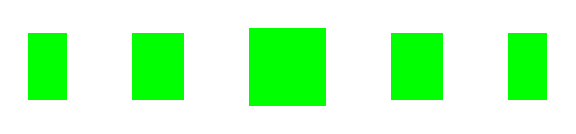
\begin{tikzpicture}[scale=3.3]
  \fill[color=green] (0, \Length - 0.13) rectangle (0.15, \Length + 0.13);
  \fill[color=green] (0.5*\Length - 0.1, \Length - 0.13) rectangle (0.5*\Length + 0.1, \Length + 0.13);
  \fill[color=green] (1.5*\Length - 0.1, \Length - 0.13) rectangle (1.5*\Length + 0.1, \Length + 0.13);
  \fill[color=green] (2*\Length - 0.15, \Length - 0.13) rectangle (2*\Length, \Length + 0.13);
  \fill[color=green] (\Length - 0.15, \Length - 0.15) rectangle (\Length + 0.15, \Length + 0.15);
  
  \LagrangeCell{0}{0}{\Length}{\Radius}{2}
    {{0,1,2,3,4,5,6,7,8}};
  \LagrangeCell{\Length}{0}{\Length}{\Radius}{4}
    {{1,9,3,49,10,5,11,12,13,14,15,16,17,18,54,19,20,21,22,23,24,25,26,27,28}};
  \LagrangeCell{0}{\Length}{\Length}{\Radius}{4}
    {{2,3,29,50,30,31,32,33,52,34,35,7,36,37,38,39,40,41,42,43,44,45,46,47,48}};
  \LagrangeCell{\Length}{\Length}{\Length}{\Radius}{2}
    {{3,49,50,51,52,53,54,55,56}};
\end{tikzpicture}

  }
  \caption{Merge on interfaces.}
\end{subfigure}
\caption[]{\textup{(continued)} Step-by-step demonstration of the enumeration algorithm for \glspl{dof} on the benchmark. Changes made at each step are highlighted. The left domain corresponds to the full mesh of the \gls{mpi} process with rank 0, the right one belongs to the one with rank 1.}
\end{figure}

\renewcommand{\thesubfigure}{\oldthesubfigure}
}
